\newpage

\question*{Digital I/O}

\begin{arabicparts}
    
    \questionpart
    With access to a DSO, the time taken to execute a digital write
    may be obtained using a program like this:
    
    \begin{lstlisting}[language=C++]
    void setup(){
        pinMode(LED_BUILTIN, OUTPUT);
    }

    void loop(){
        digitalWrite(LED_BUILTIN, LOW);
        digitalWrite(LED_BUILTIN, HIGH);
    }
    \end{lstlisting}

    The DSO probe would be connected to pin 13, corresponding to
    the LED, and ground. The time taken for the instruction will
    be half of the time period of the obtained (presumably square) wave.

    \questionpart
    We put the tested function in the \texttt{loop()} section (see Appendix)
    and then monitor the output using a C++ program with the serial output 
    pipelined into it. The C++ program was designed to count instances 
    of an arbitrary provided string and time it with a high resolution clock.
    
    The following results were obtained by timing the given program:

    \begin{figure}[ht]
        \centering
        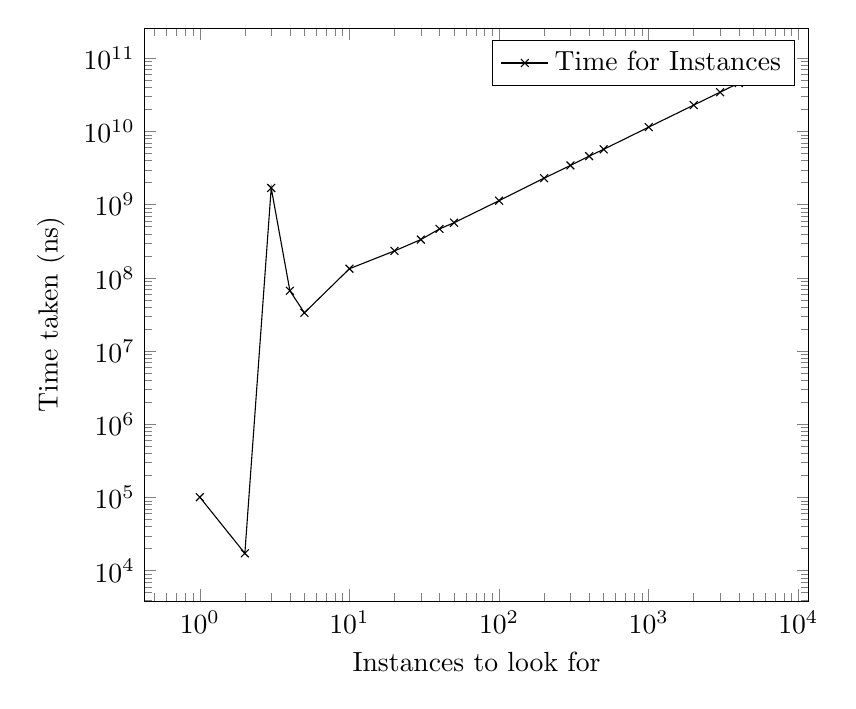
\begin{tikzpicture}

    \pgfplotsset{
        scale only axis,
    }

    \begin{axis}[
        xlabel=Instances to look for,
        ylabel=Time taken (ns),
        xmode=log,
        ymode=log
    ]
    \addplot[mark=x]
        coordinates{ % plot 1 data set
            ( 1 , 101053 )
            ( 2 , 17291 )
            ( 3 , 1.6937e+09 )
            ( 4 , 6.67496e+07 )
            ( 5 , 3.34086e+07 )
            ( 10 , 1.33625e+08 )
            ( 20 , 2.33841e+08 )
            ( 30 , 3.34033e+08 )
            ( 40 , 4.67719e+08 )
            ( 50 , 5.67789e+08 )
            ( 100 , 1.13591e+09 )
            ( 200 , 2.30494e+09 )
            ( 300 , 3.44066e+09 )
            ( 400 , 4.6101e+09 )
            ( 500 , 5.71234e+09 )
            ( 1000 , 1.14914e+10 )
            ( 2000 , 2.29831e+10 )
            ( 3000 , 3.44411e+10 )
            ( 4000 , 4.59325e+10 )
            ( 5000 , 5.74241e+10 )
        }; \label{plot_one}

        % plot 1 legend entry
        \addlegendimage{/pgfplots/refstyle=plot_one}
        \addlegendentry{Time for Instances}
    \end{axis}

\end{tikzpicture}
        \caption{Time taken to receive instances of \texttt{"01Game Over"}}
        \label{fig:timegraph}
    \end{figure}

    Looking at the figure, the first few points are quite erratic, possibly
    due many small erratic foactors interacting, such as transmission delay, serial
    poling delay, etc. The data very quickly settles into a linear plot, which
    was used to determine a best fit line of the form

    $$y = mx + c$$
    
    with obtained values,

    $$m = 1.148 \times 10^{7} \textnormal{ns}$$
    $$c = 3.907 \times 10^{5} \textnormal{ns}$$

    Thus, the average time per function run was $1.148 \times 10^{7}$ ns, i.e. \textbf{11.48 ms}.

    It is also worth noting the obtained value for $c$. There seems to be a sizable
    constant delay for each instance run. This may be attributed to the overhead
    of the timing methodology, the buffer as well as the timing program itself.
    It being a couple orders of magnitude smaller than the actual slope ensures
    that our testing methodology was appropriate and did not skew the results 
    too much. 

    {\small Note --- data for less than 10 instances was not included for the best fit.}

    {\small Actual data values and testing details may be found in the Appendix.}

\end{arabicparts}